% =====================================================================
% redes.tex
% Responsabilidad única: presentar las redes neuronales del curso
% (perceptrón, activaciones, retropropagación, perceptrón multicapa con
% parada temprana) y lo que la red aportó frente a los modelos lineales en
% ambas tareas, con el sobremuestreo y el L16.
% Cifras: macros ClfMLP*, ClfLogisticaParametros, ClfSobre*, ClfModelo*,
% RegRMSE*; figuras 05_red_*; tablas tab:clf-didactica y tab:clf-sobre.
% =====================================================================
\section{Redes neuronales: Del perceptrón al perceptrón multicapa}
\label{sec:redes}

En las dos secciones anteriores el perceptrón multicapa apareció como un
modelo más de la pasada didáctica y como un nivel del factor modelo en los
dos L16, siempre con las mismas variables, los mismos bloques y la misma
métrica que los demás. En las dos tareas perdió frente al modelo lineal y
aquí lo abrimos por dentro (cómo está hecha la red y cómo aprende) para
entender por qué.

\subsection{Del perceptrón a la red con una capa oculta}

Un perceptrón es la unidad más simple de una red. Multiplica cada entrada
por un peso, suma un sesgo y pasa el resultado por una función de activación
$\varphi$, es decir que $\hat{y}=\varphi(\mathbf{w}^\top\mathbf{x}+b)$. Si la
activación es un escalón (como en el perceptrón original) la salida es una
clase y si es la función logística $\sigma(z)=1/(1+e^{-z})$ la salida es una
probabilidad. O sea que la regresión logística de la
Sección~\ref{sec:clasificacion} es en el fondo un perceptrón de una sola
neurona entrenado con la pérdida logarítmica.

El perceptrón multicapa (MLP) mete entre las entradas y la salida una o
varias capas ocultas, cada una con sus propios pesos y una activación no
lineal. La activación es lo que le deja a la red doblar la frontera, porque
sin ella las dos capas se reducirían a una sola suma ponderada, que sería la
misma logística de antes. Con ella la red puede representar interacciones y
umbrales que un modelo lineal no captura. La red que usamos tiene una sola
capa oculta:
\begin{equation}
\mathbf{z}^{(1)}=W_1\mathbf{x}+\mathbf{b}_1,\qquad
\mathbf{h}=\operatorname{ReLU}\!\big(\mathbf{z}^{(1)}\big),\qquad
\hat{p}=\sigma\!\big(\mathbf{w}_2^\top\mathbf{h}+b_2\big),
\label{eq:mlp}
\end{equation}
donde $\hat{p}$ es la probabilidad de que la muestra resulte no conforme.

De las activaciones del curso, la logística va en la salida de un
clasificador binario porque aprieta cualquier valor entre cero y uno y la
tangente hiperbólica es su versión centrada en cero. Las dos se aplanan en los
extremos así que en las capas ocultas encogen el gradiente y la red aprende
muy despacio. La ReLU
($\max(0,z)$) deja pasar la parte positiva y anula la negativa. Como su
derivada es cero o uno no se aplana. Es la que scikit-learn usa por defecto
en las capas ocultas y la que usamos nosotros (\codigo{\ClfMLPActivacion}).

\subsection{Cómo aprende la red: Retropropagación}

La red la entrenamos con \codigo{MLPClassifier}, que en cada lote de $m$ filas
minimiza la pérdida logarítmica (que castiga darle poca probabilidad a lo que
sí pasó) más una penalización $L_2$ sobre el tamaño de los pesos, con
intensidad $\alpha$ (\codigo{alpha}, aquí \ClfMLPAlfa{}) y dividida por el
tamaño del lote:
\begin{equation}
J=-\frac{1}{m}\sum_{i=1}^{m}\Big[y_i\log\hat{p}_i+(1-y_i)\log(1-\hat{p}_i)\Big]
+\frac{\alpha}{2m}\Big(\lVert W_1\rVert^2+\lVert \mathbf{w}_2\rVert^2\Big).
\label{eq:perdida-mlp}
\end{equation}
La retropropagación calcula con la regla de la cadena cuánto cambia $J$ cuando
se mueve cada peso, capa por capa desde la salida hacia la entrada. Con una
salida logística y la pérdida logarítmica la derivada respecto de la entrada
de la neurona de salida se simplifica a $\hat{p}_i-y_i$, que es simplemente
cuánto se equivocó la red con esa muestra. Para los pesos de la capa oculta
todo queda en una sola ecuación,
\begin{equation}
\frac{\partial J}{\partial W_1}
=\frac{1}{m}\Bigg[\sum_{i=1}^{m}
\underbrace{(\hat{p}_i-y_i)}_{\partial J/\partial z^{(2)}}\;
\underbrace{\Big(\mathbf{w}_2\odot\mathbb{1}\big[\mathbf{z}^{(1)}_i>0\big]\Big)}_{\partial z^{(2)}/\partial\mathbf{z}^{(1)}}\;
\underbrace{\mathbf{x}_i^\top}_{\partial\mathbf{z}^{(1)}/\partial W_1}
+\alpha W_1\Bigg],
\label{eq:retropropagacion}
\end{equation}
donde el indicador es la derivada de la ReLU (uno si la neurona estaba
encendida y cero si no) y el término $\alpha W_1$ viene de la penalización,
que empuja los pesos hacia cero. Con ese gradiente el optimizador mueve cada
peso un paso en contra. El que usamos (\codigo{\ClfMLPOptimizador}, el de
scikit-learn por defecto) ajusta el paso de cada peso según cómo se movió su
gradiente en los lotes anteriores.

Una pasada completa por el entrenamiento se llama época. Para que la red no
memorice usamos parada temprana (\codigo{early\_stopping}): La red aparta al
azar el \ClfMLPFraccionValidacionPct{}\,\% de sus filas de ajuste, mide la
exactitud en esa fracción al final de cada época y se detiene cuando lleva
\ClfMLPPaciencia{} épocas sin mejorar, con un tope de \ClfMLPTopeEpocas{}. Así
el número de épocas funciona como una segunda regularización. Eso sí, esa
fracción se aparta al azar y no por fecha así que la parada vigila el error
dentro del mismo periodo. La comparación entre modelos, en cambio, sigue
usando los bloques temporales.

\subsection{La red que usamos y su entrenamiento}

La red tiene \ClfMLPEntradas{} entradas (las columnas que deja el
preprocesamiento del grupo ampliado), una capa oculta de \ClfMLPOcultas{}
neuronas ReLU y una salida logística (Figura~\ref{fig:red-arquitectura}). En
total son \ClfMLPParametros{} pesos y sesgos frente a los
\ClfLogisticaParametros{} coeficientes de la regresión logística con las
mismas entradas, o sea unas \ClfMLPVecesParametros{} veces más.

\begin{figure}[!htbp]
\centering
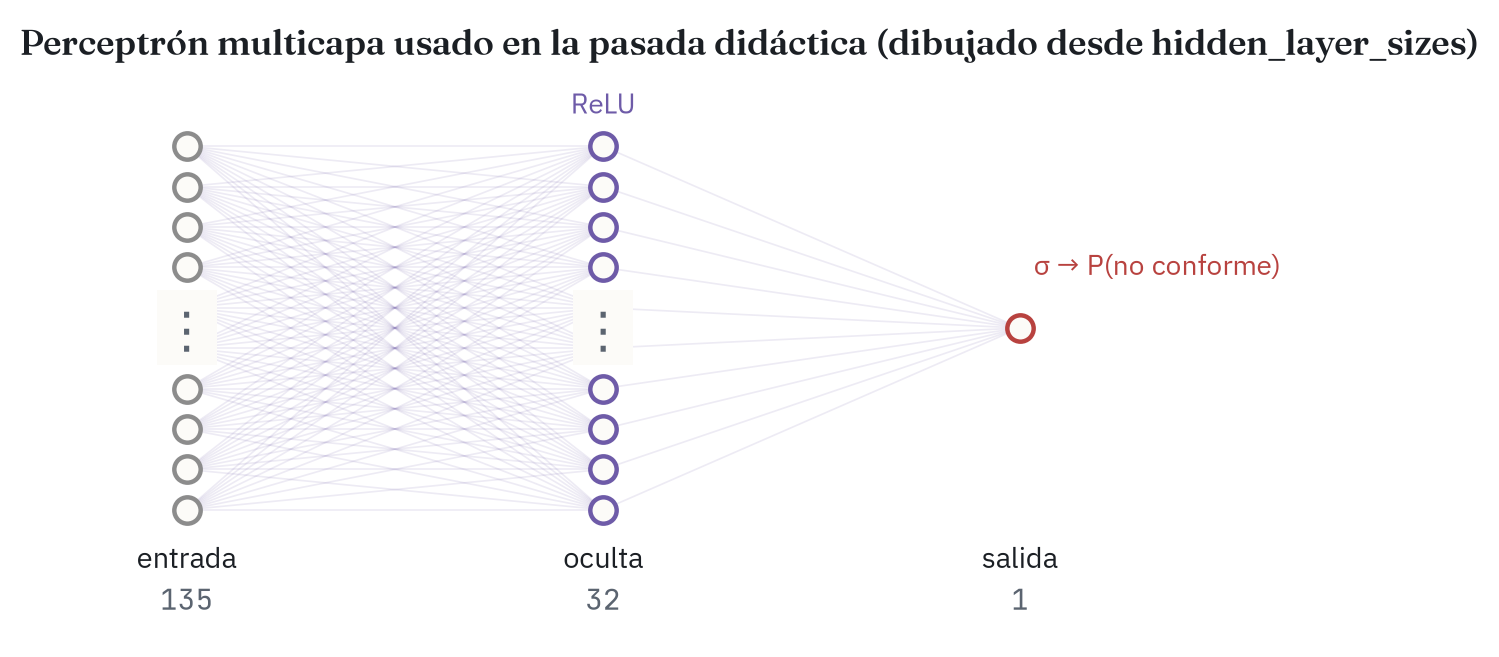
\includegraphics[width=0.52\textwidth]{04_red_arquitectura.png}
\caption{Arquitectura del perceptrón multicapa de la pasada didáctica,
dibujada desde \codigo{hidden\_layer\_sizes}: Las capas grandes se muestran
recortadas y casi todos los parámetros están en las conexiones entre la
entrada y la capa oculta.}
\label{fig:red-arquitectura}
\end{figure}

Cuando la ajustamos una vez con todo el entrenamiento la red se detuvo en la
época \ClfMLPEpocas{}, \ClfMLPPaciencia{} después de la mejor
(\ClfMLPMejorEpoca{}), como se ve en la Figura~\ref{fig:red-curvas}. La pérdida
de entrenamiento siguió bajando hasta \ClfMLPPerdidaFinal{}, mientras que la
exactitud en la fracción apartada llegó como máximo a
\ClfMLPExactitudMejor{}, apenas por encima de la que se obtiene diciendo
siempre ``conforme'' (\ClfTasaMayoritaria{}). Esto explica parte del
problema: Con tan pocas no conformes la exactitud casi no distingue un modelo
que ordena bien de uno que no así que la parada temprana de scikit-learn
está vigilando una señal muy débil. Por eso en todo el proyecto comparamos
los modelos con el ROC-AUC y no con la exactitud.

\begin{figure}[!htbp]
\centering
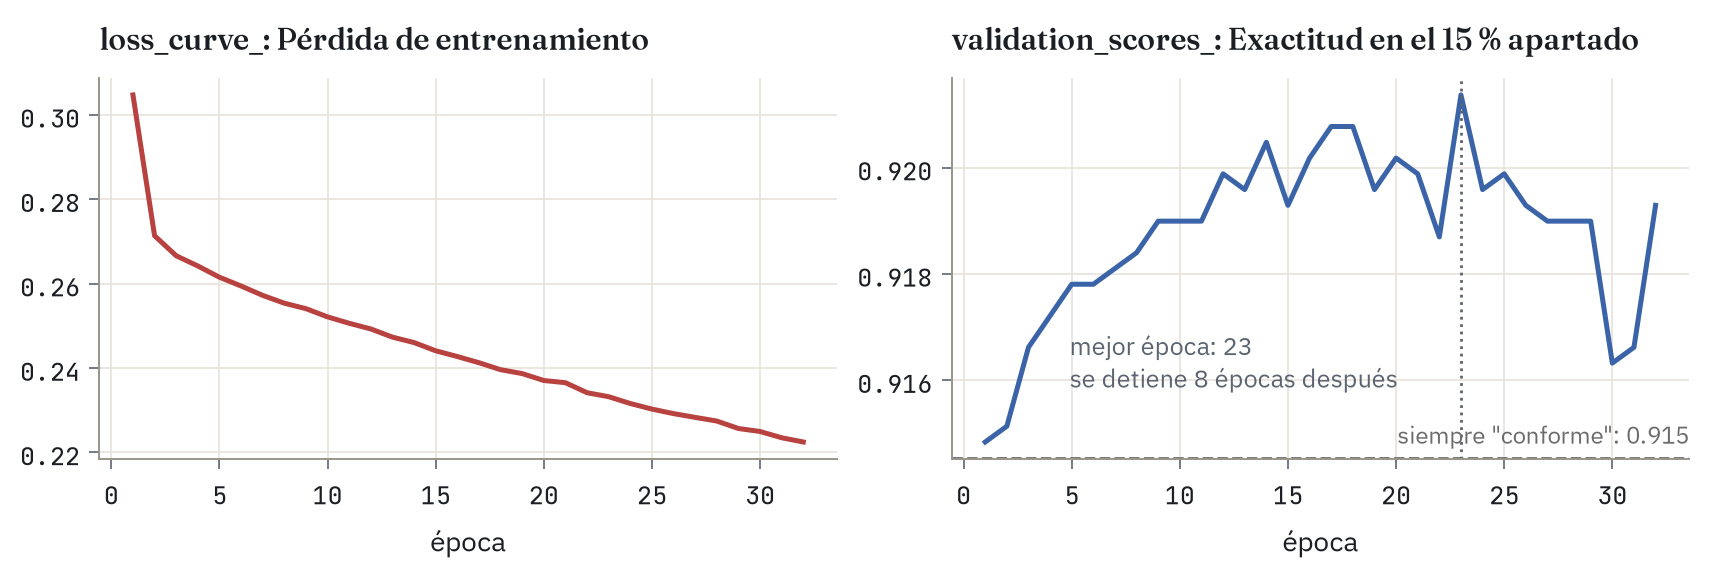
\includegraphics[width=0.84\textwidth]{04_red_curvas.png}
\caption{Curvas de la red ajustada con todo el entrenamiento, con la pérdida
logarítmica por época (\codigo{loss\_curve\_}) y la exactitud en la fracción
apartada (\codigo{validation\_scores\_}): La pérdida sigue bajando mientras
la exactitud se queda pegada a la de responder siempre ``conforme''
(discontinua) y la punteada marca la mejor época.}
\label{fig:red-curvas}
\end{figure}

\subsection{Qué aportó la red frente a los modelos lineales}

La respuesta corta es que en estos datos no le ganó al modelo lineal. En clasificación la red obtuvo
en la pasada didáctica un ROC-AUC medio de \ClfAUCMLPDidactico{} frente a
\ClfAUCLogisticaDidactico{} de la regresión logística
(Tabla~\ref{tab:clf-didactica}) y en regresión un RMSE medio de
\RegRMSEMLPDidactico{} frente a \RegRMSELinealDidactico{} de la regresión
lineal múltiple (Tabla~\ref{tab:reg-didactica}). Le dimos varias vueltas a si
una red más grande o con menos penalización ordenaría mejor y en la regresión
la rejilla tampoco cambió el orden (\RegRejillaMLPRMSE{} frente a
\RegRejillaLinealRMSE{}). O sea que pese a tener muchos más parámetros la red
no mejora al modelo lineal en ninguna de las dos tareas. Nuestra lectura es
que en estos datos simulados la señal está sobre todo en efectos que se suman
(en la escala de la carga o en la del logit) y que el modelo lineal ya los
captura así que la capa oculta no encuentra interacciones que compensen lo que
cuesta en varianza y en interpretación ya que la red no da razones de odds
que se puedan leer.

El sobremuestreo agrava la diferencia. Es al
\MakeLowercase{\ClfSobreMasPierde} al que más ROC-AUC le quita
(\ClfSobreDeltaAUC{}, Tabla~\ref{tab:clf-sobre}), mientras que a la
\MakeLowercase{\ClfSobreMenosPierde} casi no la cambia
(\ClfSobreDeltaAUCMenor{}). Una explicación posible, que no comprobamos por
separado, es que el sobremuestreo aleatorio repite filas no conformes que una
red con \ClfMLPParametros{} parámetros puede memorizar. Además las copias de
una misma fila pueden caer a la vez en la parte de ajuste y en la fracción
que vigila la parada temprana, de modo que la parada deja de notar el
sobreajuste. La logística, con \ClfLogisticaParametros{} coeficientes, casi
no tiene cómo memorizar.

El L16 de clasificación cuenta lo mismo desde otro diseño: En el
factor \ClfFactorPrincipal{} el mejor nivel es la \ClfModeloMejorNivel{} (S/N
media de \ClfSNModeloMejor{} dB) y el peor el \ClfModeloPeorNivel{}
(\ClfSNModeloPeor{} dB). Como cada nivel se promedia sobre corridas con y sin
sobremuestreo, parte de esa diferencia viene de lo que el sobremuestreo le
hace a la red. Con datos reales podría haber interacciones
que el generador no tiene así que antes de descartar la red repetiríamos la
comparación.
